%-------------------------------------------------------------------------------------------
\documentclass[aspectratio=169,UTF8,11pt]{ctexbeamer}

%%%%%%%%%%%%%%%%%%%%%%%%%%%%%
\usepackage{colortbl}
\usepackage{color}
\usepackage{booktabs}
\usepackage{threeparttable}
\usepackage{hyperref}
%\usepackage{babel}
%%%%%%%%%%%%%%%%%%%%%%%%%%%%%

\mode<presentation> {
\usetheme{Madrid}
%\setbeamertemplate{footline} % To remove the footer line in all slides uncomment this line
\setbeamertemplate{footline}[frame number] % To replace the footer line in all slides with a simple slide count uncomment this line
\setbeamercolor{page number in head/foot}{fg=blue}
\setbeamertemplate{navigation symbols}{} % To remove the navigation symbols from the bottom of all slides uncomment this line
}

% User Defined Block %%%%%%%%%%%%%%%%%%%%%%%%%%%%%%%%%%%%%%%%%%%%%%%%%%%%%%%%
\usepackage{setspace}
\definecolor{orange}{rgb}{1,0.5,0}
\definecolor{aa}{RGB}{34,139,34}
\definecolor{lightblue}{rgb}{0,0.85,0.9}
\definecolor{darkblue}{rgb}{0,0.7,1}

\definecolor{hanblue}{rgb}{0.27, 0.42, 0.81}
\definecolor{indiagreen}{rgb}{0.07, 0.53, 0.03}
\definecolor{indianred}{rgb}{0.8, 0.36, 0.36}
\definecolor{indianyellow}{rgb}{0.89, 0.66, 0.34}
\definecolor{babypink}{rgb}{0.96, 0.76, 0.76}
\definecolor{ao(english)}{rgb}{0.0, 0.5, 0.0}
\setbeamerfont{block title}{size=\normalsize}
\setbeamerfont{block body}{size=\small}

\newenvironment<>{blueblock}[1]{%
  \setbeamercolor{block title}{fg=white,bg=hanblue}%
  \begin{block}#2{#1}}{\end{block}}

\newenvironment<>{greenblock}[1]{%
  \setstretch{1.3}\setbeamercolor{block title}{fg=white,bg=indiagreen}%
  \begin{block}#2{#1}}{\end{block}}

\newenvironment<>{redblock}[1]{%
  \setstretch{1.3}\setbeamercolor{block title}{fg=white,bg=indianred}%
  \begin{block}#2{#1}}{\end{block}}

\newenvironment<>{yellowblock}[1]{%
  \setstretch{1.3}\setbeamercolor{block title}{fg=white,bg=indianyellow}%
  \begin{block}#2{#1}}{\end{block}}

%----------------------------------------------------------------------------------------
%	PACKAGES
%----------------------------------------------------------------------------------------
\usepackage{graphicx} % Allows including images
%\usepackage{tikz}
%\usetikzlibrary{shapes.geometric, arrows}
\usepackage{listings}
\lstset{language=C++,
    columns=flexible,
   % basicstyle=\scriptsize\ttfamily,                                      % 设定代码字体、大小4
    basicstyle=\footnotesize\ttfamily,
    %numbers=left,xleftmargin=2em,framexleftmargin=2em,                   % 在左侧显示行号
    %numberstyle=\color{darkgray},                                        % 设定行号格式
    keywordstyle=\color{blue},                                            % 设定关键字格式
    commentstyle=\color{ao(english)},                                     % 设置代码注释的格式
    stringstyle=\color{brown},                                            % 设置字符串格式
    %showstringspaces=false,                                              % 控制是否显示空格
	%frame=lines,                                                         % 控制外框
    breaklines,                                                           % 控制是否折行
    postbreak=\space,                                                     % 控制折行后显示的标识字符
    breakindent=5pt,                                                      % 控制折行后缩进数量
    emph={size\_t,array,deque,list,map,queue,set,stack,vector,string,pair,tuple}, % 非内置类型
    emphstyle={\color{teal}},
    escapeinside={(*@}{@*)},
}
%---------------------------------------------------------------------------------------------------

%%%%%%%%%%%%%%%%%%%%%%%%%%%%%%%%%%%%%%%%%%%%%%%%%%%%%%%%%%%%%%%%%%%%%%%%%%%%%%%%%%%%%%%%%%%%%%
\title[\textit{计算机程序设计基础}]{计算机程序设计基础}
\author[李长河]{李长河} % Your name
\institute[CUG] % Your institution as it will appear on the bottom of every slide, may be shorthand to save space
{
中国地质大学(武汉)自动化学院\\ % Your institution for the title page
\medskip
\textit{lichanghe@cug.edu.cn} % Your email address
}
\date{2021年3月} % Date, can be changed to a custom date
%%%%%%%%%%%%%%%%%%%%%%%%%%%%%%%%%%%%%%%%%%%%%%%%%%%%%%%%%%%%%%%%%%%%%%%%%%%%%%%%%%%%%%%%%%%%%%


\begin{document}
\maketitle
%\begin{frame}[noframenumbering]           %beamer里重要的概念,每个frame定义一张page
%\centering
%{\large 李长河 \vspace{0.5cm} \\自动化学院710 \vspace{0.5cm}\\ lichanghe@cug.edu.cn}
%\end{frame}

%-----------------------------------------------------------


\addtocounter{framenumber}{-1}
%---------------------------------------------------------------------------------------------
\begin{frame}{目录}
	\tableofcontents
\end{frame}

%---------------------------------------------------------------------------------------------
\begin{frame}[fragile]{~} % Table of contents slide, comment this block out to remove it
\begin{block}{学习目标}
\begin{enumerate}
  \item 掌握 C++ 程序的基本组成、了解类的概念;
  \item 学会独立上机编写、调试以及运行一个简单的 C++ 程序。
\end{enumerate}
\end{block}
\end{frame}

%%%%%%%%%%%%%%%%%%%%%%%%%%%%%%%%%%%%%%%%%%%%%%%%%%%%%%%%%%%%%%%%%%%%%%%%%%%%%%%%%%%%%%%%%%%%%%
\section{编写一个C++程序}
%%%%%%%%%%%%%%%%%%%%%%%%%%%%%%%%%%%%%%%%%%%%%%%%%%%%%%%%%%%%%%%%%%%%%%%%%%%%%%%%%%%%%%%%%%%%%%

%---------------------------------------------------------------------------------------------
\begin{frame}[fragile]{1.1 编写一个C++程序}
\begin{columns}
\column{0.9\textwidth}
\begin{blueblock}{一个空的main函数}
\vspace{-3mm}
\begin{lstlisting}
/*    一个空的main函数,    返回一个整型值
*/
int main(){     //程序从main函数开始执行
    return 0;   /*返回一个整型值*/
}
\end{lstlisting}
\vspace{-4mm}
\end{blueblock}

\begin{yellowblock}<2->{注释}
\vspace{-2mm}
	\begin{itemize}
        \item \texttt{main()}是主函数,也是入口函数
		\item 函数包括四部分:返回值类型、函数名、形参列表和函数体
        \item \texttt{int}(整型类型),即为\texttt{main}函数返回值类型
        \item \texttt{C++}有两种注释方法
            \begin{itemize}
                \item 双斜线\texttt{(//)}注释单行语句,以换行符结束
                \item 界定符\texttt{(/*~*/)}注释多行语句,以\alert{\texttt{/*}}开始,到\alert{\texttt{*/}}结束
            \end{itemize}
	\end{itemize}
\end{yellowblock}
\end{columns}
\end{frame}

%---------------------------------------------------------------------------------------------
\begin{frame}[fragile]{1.1 编写一个C++程序}
\begin{greenblock}{例1.2}
  已知圆柱体的底面半径和高分别为6cm和12cm,求圆柱体的体积?
\end{greenblock}
\pause
\begin{columns}[t]
\column{0.8\textwidth}
\begin{greenblock}{数学解法}
\begin{spacing}{1.5}
~\\
\texttt{解:设半径为radius,高为height,体积为volume\\
~~~~~~由已知可得:radius=6cm,height=12cm\\
~~~~~~volumn=$\pi$*radius$^{2}$*height=3.14*6*6*12=1356.48cm$^{3}$。}
\end{spacing}
\end{greenblock}
\end{columns}
\end{frame}

%---------------------------------------------------------------------------------------------
\begin{frame}[fragile]{1.1 编写一个C++程序}
\vspace{-6mm}
\begin{columns}[t]
\column{0.65\textwidth}
\begin{greenblock}{代码清单1.2,例1.2}
\vspace{-3mm}
\begin{lstlisting}
#include <iostream>
int main() {
    // 定义三个double类型对象,存放半径、高和体积的值
    double radius, height, volume;
    //屏幕终端显示Please input radius and height:
    std::cout << "please input radius and height: ";
    //从键盘输入6.5 12回车
    std::cin >> radius >> height;
     //计算圆柱体体积,并把结果存放到对象volume中
    volume = 3.14*radius*radius*height;
    //屏幕输出 the volume is 1591.98
    std::cout << "the volume is " << volume;
    return 0;
}
\end{lstlisting}
\end{greenblock}
\column{0.3\textwidth}
	\begin{yellowblock}<2->{注释}
		\begin{itemize}
			\item iostream为输入输出流库,通过cin和cout语句来实现读写操作
            \item “std::”表明cin、cout定义在std的命名空间,“::”为作用域运算符
            \item radius、 height和 volume均为double类型的对象
		\end{itemize}
	\end{yellowblock}
\end{columns}
\end{frame}

%%%%%%%%%%%%%%%%%%%%%%%%%%%%%%%%%%%%%%%%%%%%%%%%%%%%%%%%%%%%%%%%%%%%%%%%%%%%%%%%%%%%%%%%%%%%%%
\section{认识类}
%%%%%%%%%%%%%%%%%%%%%%%%%%%%%%%%%%%%%%%%%%%%%%%%%%%%%%%%%%%%%%%%%%%%%%%%%%%%%%%%%%%%%%%%%%%%%%

%---------------------------------------------------------------------------------------------
\begin{frame}[fragile]{1.2 认识类}
\begin{columns}[t]
\column{0.9\textwidth}
\alert{类(class)=数据结构(data structure)+ 操作(algorithm)}
~\\
~\\
\begin{block}{类(class)}
~\\
    \begin{itemize}
    \begin{spacing}{1.5}
        \item 核心思想是定义一种数据结构(data structure)以及与数据结构相关联的一组操作,并把它们封装在一起,形成一个\alert{类类型}(class type)。
        \item 属于用户自定义类型,具有抽象(abstract)和封装(encapsulation)的属性,是面向对象程序设计(object-oriented programming, OOP)的基础。
    \end{spacing}
		\end{itemize}
\end{block}
\end{columns}

\end{frame}

%---------------------------------------------------------------------------------------------
\begin{frame}[fragile]{1.2 认识类}
下面用面向对象的方法来求解前面的求圆柱体体积的问题
\vspace{-3mm}
\begin{columns}[t]
\column{0.6\textwidth}
\begin{blueblock}<2->{代码清单 1.3,例1.3}
\vspace{-3mm}
\begin{lstlisting}
#include<iostream>
using namespace std;    //使用标准命名空间
class Cylinder {    //定义一个名为Cylinder的类类型
    double m_radius, m_height;
public:
    double volume() {   //计算圆柱体的体积
        return 3.14*m_radius*m_radius*m_height;
    }
    Cylinder(double i=0, double h=0) :m_radius(i), m_height(h){}    //初始化半径和高的操作
};
int main() {
    Cylinder object(1.0, 1.0);   //定义并初始化对象object
    double vol=object.volume();  //调用类成员volume函数
    cout << vol << endl;
}
\end{lstlisting}
\end{blueblock}

\column{0.35\textwidth}
\begin{yellowblock}<3->{注释}
		\begin{itemize}
            \item \texttt{Cylinder}为自定义的类类型,其定义了一个含有半径和高的数据结构以及与之关联的操作。
            \item 此处\texttt{cout}没有\texttt{std::}前缀是因为通过\texttt{using namespace std;}提前声明了使用标准命名空间。
		\end{itemize}
\end{yellowblock}

\end{columns}
\end{frame}

%%%%%%%%%%%%%%%%%%%%%%%%%%%%%%%%%%%%%%%%%%%%%%%%%%%%%%%%%%%%%%%%%%%%%%%%%%%%%%%%%%%%%%%%%%%%%%
\section{编译与调试程序}
%%%%%%%%%%%%%%%%%%%%%%%%%%%%%%%%%%%%%%%%%%%%%%%%%%%%%%%%%%%%%%%%%%%%%%%%%%%%%%%%%%%%%%%%%%%%%%

%---------------------------------------------------------------------------------------------
\begin{frame}[fragile]{1.3 编译与调试程序}
\begin{center}
    \textcolor{blue}{\texttt{C++}程序编译、调试和执行步骤}
\end{center}
\vspace{-5mm}
\pause
\begin{columns}[t]

\column{0.4\textwidth}
\begin{figure}[!h]
\centering
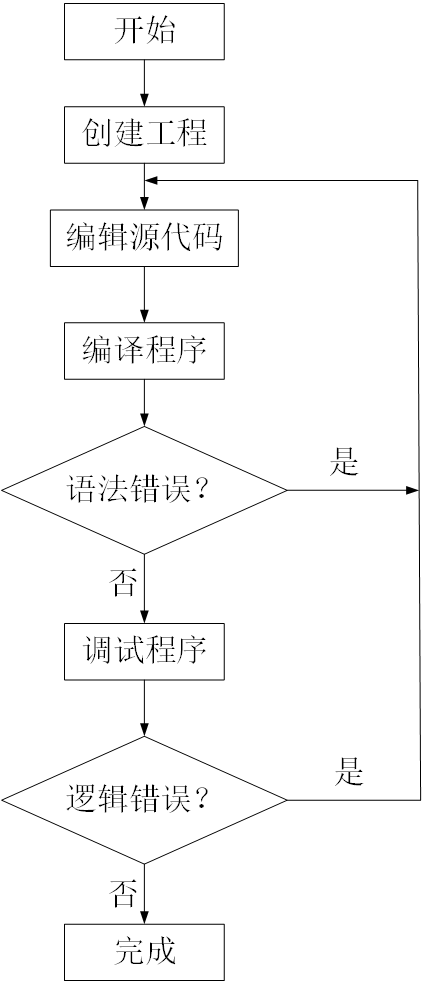
\includegraphics[width=2.8cm]{debug_flowchart}
\end{figure}
\pause
\column{0.5\textwidth}
\begin{yellowblock}{说明}
\begin{enumerate}
  \item \texttt{C++}程序工程的创建\\推荐使用\alert{\texttt{Visual Studio}}编译器
  \item 添加空的源文件\texttt{(*.cpp)},如\texttt{main.cpp}
  \item 编写源代码
  \item 编译,编译器会指出具体的语法错误
  \item 改正语法错误
  \item 调试程序(找出逻辑错误)
  \item 运行程序
\end{enumerate}
\end{yellowblock}

\end{columns}
\end{frame}


%---------------------------------------------------------------------------------------------
\begin{frame}[fragile]{1.3 编译与调试程序}

\begin{columns}[t]
\column{0.8\textwidth}
\begin{blueblock}{\texttt{Visual Studio}几个常用快捷键}
\begin{tabular}{ll}
  % after \\: \hline or \cline{col1-col2} \cline{col3-col4} ...
  \alert{\texttt{F5}} & 执行程序 \\
  \alert{\texttt{F7}} & 编译源文件 \\
  \alert{\texttt{F9}} & 添加断点 \\
  \alert{\texttt{F10}} & 单步执行一行代码 \\
  \alert{\texttt{Ctrl+F5}} & 执行但不调试 \\
\end{tabular}
\end{blueblock}
\pause
~\\
\begin{yellowblock}{建议}
	\begin{itemize}
		\item 遵循“编辑--编译--调试”的原则
		\item 养成调试程序的好习惯
	\end{itemize}
\end{yellowblock}

\end{columns}
\end{frame}


%---------------------------------------------------------------------------------------------
\begin{frame}[fragile]{课后作业}

\begin{columns}[t]
\column{0.8\textwidth}
\begin{blueblock}{作业本}
 \begin{enumerate}
   \item 教材p7:1.1 和 1.5
 \end{enumerate}

\end{blueblock}

\begin{blueblock}{上机练习}
 \begin{enumerate}
   \item 实验指导书:实验一
 \end{enumerate}

\end{blueblock}
\end{columns}
\end{frame}


%---------------------------------------------------------------------------------------------
\begin{frame}[fragile]
	\frametitle{~~}
	\begin{center}
		\huge{本章结束}
	\end{center}
\end{frame}

\end{document}
